\section{Network Structures}

Just like stock markets and airline routes, the cyber-insurance market can be described using graphs. The structure it takes are dependent on all the nodes and how they connect with each other. The way they choose to connect can be manipulated by the insurer, which will is the purpose of our modeling work. However, first we need to shield light on what kind of graph structures that would be desirable to force upon the cyber-insurance market.

To find the proper structure, many different scenarios needs to be covered. In the network a node's actions are influenced by their neighborhood structure, i.e. the network connections will affect each individual nodes payoff. Meaning that nodes are dependent on each other, and the probability of cascading failures are highly relevant. -If one or more fail, e.g. bankruptcy, failure to deliver at the expected time, higher cost etc. Then the whole network will be affected. In this case there are several types of networks to consider, all social and economic interactions where an agents well being is dependent on externalities as well as their own actions, is a network worth considering.


We found several interesting papers originated in evolutionary studies and disease contagion, which described the different characteristics in certain graph structures. More general results describing the benefits from star-shaped graphs and cliques where found. In common they showed characteristics which could be used to make it feasible for both the insurer to offer - and the customer to acquire insurance. In addition papers describing network formation processes was in particular interest for our modeling work. 

 The paper \cite{lieberman2005evolutionary} is about evolutionary dynamics and how some structures
can amplify or sustain evolution and drift\footnote{Drift is the opposite of selective evolution
, it is when the network/structure evolve and change at random}. One aspect of cyber-insurance is risk, and knowledge of how for example viruses spread in a network and how to use graph structures to prevent malicious hackers from entering your network is important. Evolutionary dynamics, and the research of how mutant genes spread though out a population as described in the paper is analogous to this issue.
If we can determine some structures, where certain nodes are advantageous/disadvantageous, then these structures will have properties, such as sustaining viruses from spreading, or amplify the incentive for obtaining cyber-insurance. 

In the \cite{lieberman2005evolutionary} paper, they show that mutants inserted in to a
 circulation graph, will have a fixation probability equal to
\begin{equation}  
p_{1}=\frac{(1-\frac{1}{r})}{(1-\frac{1}{r^{N}})}
 \label{eq:fixation} 
\end{equation}
Where $r$ represents the relative fitness of the mutant, if it is advantageous it will have a certain chance of fixation, and disadvantageous mutants will have a chance of extinction. 
A circulation graph is a graph that satisfy these two properties: 
\begin{enumerate}
\item The sum of all edges leaving a vertex is equal for all vertexes
\item The sum of all edges entering a vertex i equal for all vertexes
\end{enumerate}
I.e. a clique is a circulation graph, and the probability of fixation is as in Eq. (\ref{eq:fixation}).
The fixation probability determines how probable it is that the whole network will eventually be
"infected" by the mutant. It determines the rate of evolution, which relies on both the size of the
network and the evolution speed. 
If the relative fitness of the nodes are high, then the probability of fixation will be low.
A probability equal to one means that every node in the network eventually will be affected by the mutant.

An essential part of cyber-insurance is for the insurer to be able to calculate the overall risk of the instance requesting to be insured. 
As we shall see there are structures which will provide a higher utility than circulation graphs, however since the probability of fixation can be calculated, it will be easier for the insurer to calculate the risk. If we can find graphs with fixation probability that exceeds Eq.(\ref{eq:fixation}) it would be possible to further suppress drift and amplify selection and visa versa. 
\begin{figure}[b]
\centering
\begin{tabular}{@{}c@{}}
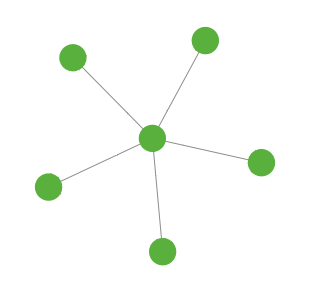
\includegraphics[width=0.5\textwidth]{../Figures/aStar.png}
\end{tabular}
\caption{
\label{fig:star} A star-topology. 
}
\end{figure}
The paper shows that there exists such graphs, one example is the star topology, (see Figure \ref{fig:star}).
In this topology the fixation probability is as shown in Eq.(\ref{eq:fixation2}), or for more general see Eq.(\ref{eq:fixationk}). \begin{equation}p_{2}=\frac{(1-\frac{1}{r^{2}})}{(1-\frac{1}{r^{2N}})} \label{eq:fixation2} \end{equation}.
or more generall: \begin{equation}
p_{k}=\frac{(1-\frac{1}{r^{k}})}{(1-\frac{1}{r^{kN}})} \label{eq:fixationk}
\end{equation}
 When comparing the Eq.(\ref{eq:fixation}) and Eq.(\ref{eq:fixation2}), we see that the selective difference is
 amplified from $r$ to $r^{2}$, i.e. a star act as an evolutionary amplifier, favoring advantageous
  mutants and inhibiting disadvantageous mutants.

There exists other graphs where the fixation probability is equal to \ref{eq:fixationk}, examples are super-stars, such as funnels and
metafunnels. These are just more complex star networks. This paper shows, that as N get large, the super-stars will have fixation probability, for an advantageous mutant, that converges to 1, and for disadvantageous converges to 0. 
As exemplified earlier in this chapter, we know that there are many
topologies in our society that are so called scale-free graphs. These graphs have most of their connectivity clustered in a few verities, which are very similar to a star, and these networks can also be considered as potent selection amplifiers. 


\subparagraph{Benefits of cliques}
The paper \cite{contagion} present interesting results regarding network formation games. 
They set up a game where the nodes benefit from direct links, but these links also expose them for risk. 
Each node gains a payoff of $a$ per link it establishes, but it can establish a maximum of $\delta$ links.
A failure occur at a node with probability $q$, and propagates on a link with probability $p$. If a node fail, it will receive a negative payoff of $b$, no matter how many links it has established. The characteristics of this game is transferable to how we expect nodes in a cyber-insurance network will interact with each other. Therefore the results of how the overall payoff changes according to different collection of participants. 
The results from their model shows a situation where clustered graphs achieve a higher payoff when connected to trusted nodes, compared to when connecting with random nodes. Unlike in anonymous graphs, where nodes connect to each other at random, nodes in these graphs share some information with their neighbors, which is used when deciding whether to form a link or not. 
To further explain these results, they show that there exists a critical point, called \textit{phase transition}, which occurs when nodes have a node degree of $\frac{1}{p}$. 
At this point a node gets a payoff of $\frac{a}{p}$, and to further increase the payoff the node needs to go into a region with significantly higher failure probability. 
Because once each node establish more than $\frac{1}{p}$ links, the contagious edges, will with high probability form a large cluster. Which results in a rise in probability of node failure, and reduces the overall welfare.
From this the paper say that when the minimum welfare exceeds 
$(1+f(\delta)*\frac{a}{p})$
we have reached super critical payoff. Otherwise it is called sub-critical payoff. 
Further they show that the only possible way of ending up with super critical payoff, is by forming clustered networks consisting of cliques with slightly more than $\frac{1}{p}$ nodes. 
However, if the nodes form an anonymous market, by random linking, they can only get sub-critical payoff. 
In other words, if the nodes can choose who they connect with, and by doing so, creating trusted clustered markets, they can achieve a higher payoff, by exceeding the critical node degree point. 


\subparagraph{Star-network as an insurable topology}
The paper \cite{networkgames} shows how network games evolve when the payoffs are determined not only by your own decisions, but also by your neighbors. This can be used to analyze the star network further. They analyze a game on public good, which is simple but highly relevant for our work. A good example of a public goods is security product. A security product suffers from strategic substitutes, i.e. if your neighbor acquire the security product, you have less incentive of also acquiring the security product. This is because when he acquire it, he gets more secure, and so do you, due to the positive externalities of the product.

The game is set up like this:
We have an action space: $X=\{0,1\}$, where 1 can be considered as acquiring information, take vaccine, buy security software etc. And 0 is not doing so.
Each node $i$ has a set of neighbors: $N_{i} $, and a payoff function $y_{i}=x_{i}+\bar{x}N_{i}$. 
The gross payoff to player $i$ is 1 if $y_{i}>=1$ and 0 otherwise. But each player also suffer from a cost of $0<c<1$ if they choose action 1.
%% [location]h-here, t top, b bottom.
\begin{figure}[h]
\centering
\begin{subfigure}{.4\textwidth}
  \centering
  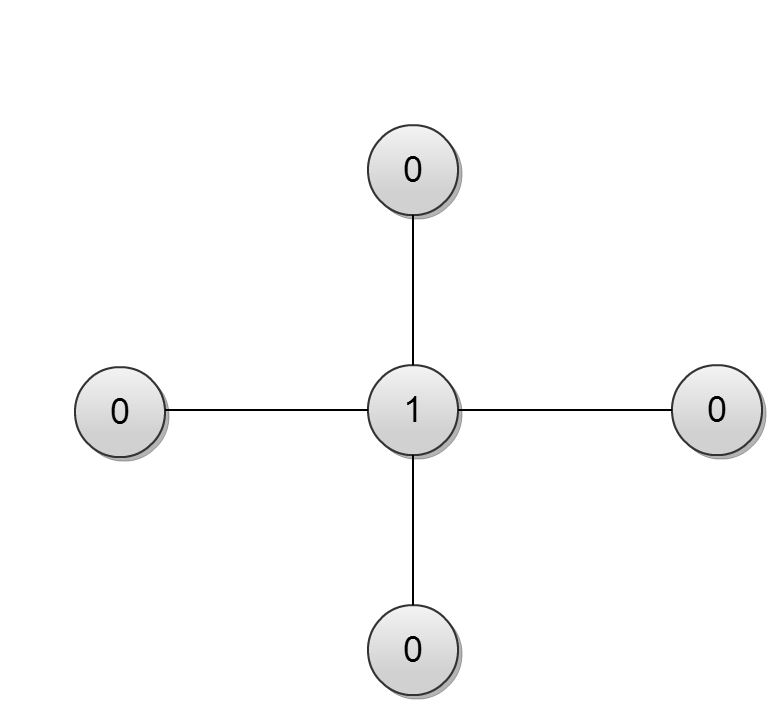
\includegraphics[width=0.8\linewidth]{optimalequilibrium.png}
  \caption{\label{fig:optequi} Socially Optimal equilibrium, center node choose action 1}
\end{subfigure}
\quad
\begin{subfigure}{.4\textwidth}
  \centering
  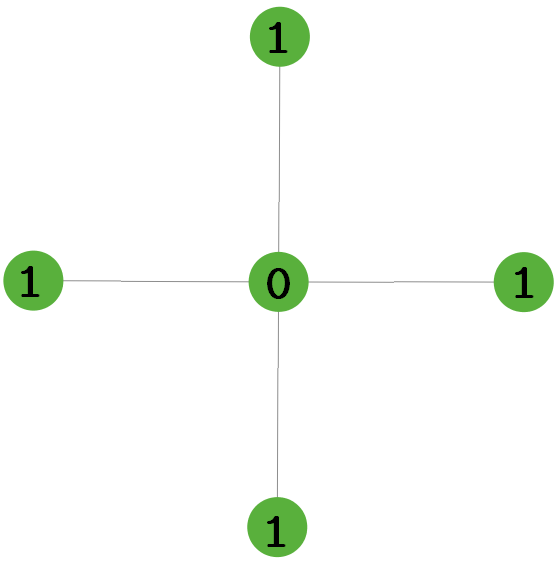
\includegraphics[width=0.8\linewidth]{notoptimalequilibrium.png}
  \caption{\label{fig:notoptequi} Non Socially Optimal equilibrium, leaf nodes choose action 1}
\end{subfigure}
\caption{\label{fig:starequi} Figure \ref{fig:optequi} shows the socially optimal equilibrium, and Figure \ref{fig:notoptequi} shows the non optimal equilibrium.}

\end{figure}
When looking at Figure \ref{fig:starequi}, we easily see that there is two equilibriums. One where the center node choose action 1 and the rest of the nodes choose action 0, and a second equilibrium where all the leaf nodes chooses 1 and the center choose 0.
The overall payoff in these two differ from each other, the latter is not socially optimal because it
 suffers from a cost equal to: $\#leaf nodes*c$, while the other equilibrium only have a total cost of $c$.
 It would have been beneficial if we where able to force the game to always end up in the social optimal equilibrium.


\subparagraph{From a insurers point of view}
If a insurance company could identify these star-structures, and force them to end up in the social optimal equilibrium it would have been very beneficial for both the insurer and the customers.
First of all if the insurer could identify these structures, he could calculate the overall probability of fixation by a diseased mutant(virus, worm, trojan or other failures) as shown earlier. If they could ensure that the center node is protected they could also calculate the probability of the diseased mutant being extinguished from the network.
One possibility of achieving this could be by offering very cheap insurance to the leaf nodes, and giving the center node an incentive to acquire security product, by informing the center node about the probability of failure unless he acquires security. And offer him a very good rebate if acquire the security product, and a very expensive insurance if not. In this way the insurer could force a rational center node to getting both insurance and security product, and thus securing the whole network.

This is a simple scenario, analyzing an exogenous network formation \footnote{Exogenous: The network formation is given. Endogenous: The structure originates from within the network, i.e. the opposite of exogenous}, 
but it shows how a insurer can, by using the results from \cite{lieberman2005evolutionary}, force the game to end up in the social optimal equilibrium, and also how the insurer can calculate the probabilities of failure. 
The contributes significantly to solving some of the problems with cyber-insurance. The problems with information asymmetry and interdependent risk problem has been reduced, since if the insurer knows the network structure, he can calculate the probabilities of failures and catastrophic events, the most important information he needs is how secure the center node is. If he also can ensure that the center node is secure, the interdependent risk problem is limited to only one node, the center node. 

   
